\documentclass[UTF8]{ctexbeamer}
\usepackage{latexsym,amsmath,xcolor,multicol,booktabs,calligra,heuristica,tikz,graphicx,amssymb,amsfonts,amsmath,makeidx}
\usepackage{bbding}
\usepackage{graphicx}
\usetheme{Pittsburgh}
\usecolortheme{beaver}
\newcommand{\cndash}{\rule{0.2em}{0pt}\rule[0.35em]{1.6em}{0.05em}\rule{0.2em}{0pt}}
\AtBeginSection[]
{
  \begin{frame}<beamer>{目录}
    \tableofcontents[currentsection]
  \end{frame}
}
\begin{document}
\begin{frame}
    \title{\kaishu{数学学术写作} \\ Mathematical Writing}
    \author{东林, 石雨凌}
    \titlepage
    \date{\today}
\end{frame}   
\section{前言}

\begin{frame}{关于 Paul Erdos}
    \textit{A mathematician, is a machine for turning coffee into theorems.     \\ \ \\ 数学家, 是将咖啡转换成定理的机器。}
        \flushright{\cndash Paul Erdos} 
\end{frame}

\begin{frame}{关于 Paul Erdos}
\begin{alertblock}{发表论文最多的数学家}
Erdõs Pál(1913-1996), 生于匈牙利, 研究兴趣广泛, \textit{Mathematical Reviews} 曾把数学划分为大约六十个分支,Erdos的论文涉及到了其中的40\%, 一生中同500余位合作者发表过逾1500篇数学论文.
\end{alertblock}
    \begin{figure}
        \centering
        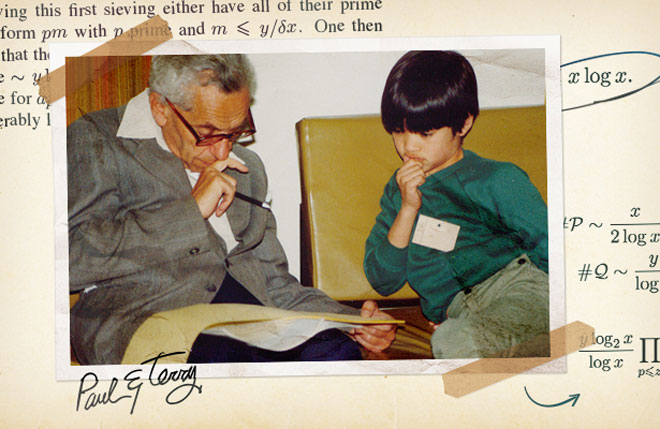
\includegraphics[width=0.65\textwidth]{figure/erdosWithTao.jpg}
        \caption{Erdos 与 Terence Tao讨论}
        \label{fig:my_label}
    \end{figure}
\end{frame}

\begin{frame}{关于 Paul Erdos}
\begin{alertblock}{Erdos数}
Erdos本人计做0,与Erdos合作过的计做1。与Erdos数为1的人合作过的人计做2,以此类推,不属于以上任何一类的就是 $\infty$。谨举几例:物理学家费米的Erdos数是3,海森堡是4,爱因斯坦是2,比尔.盖茨的Erdos数是4。
\end{alertblock}
    \begin{figure}
        \centering
        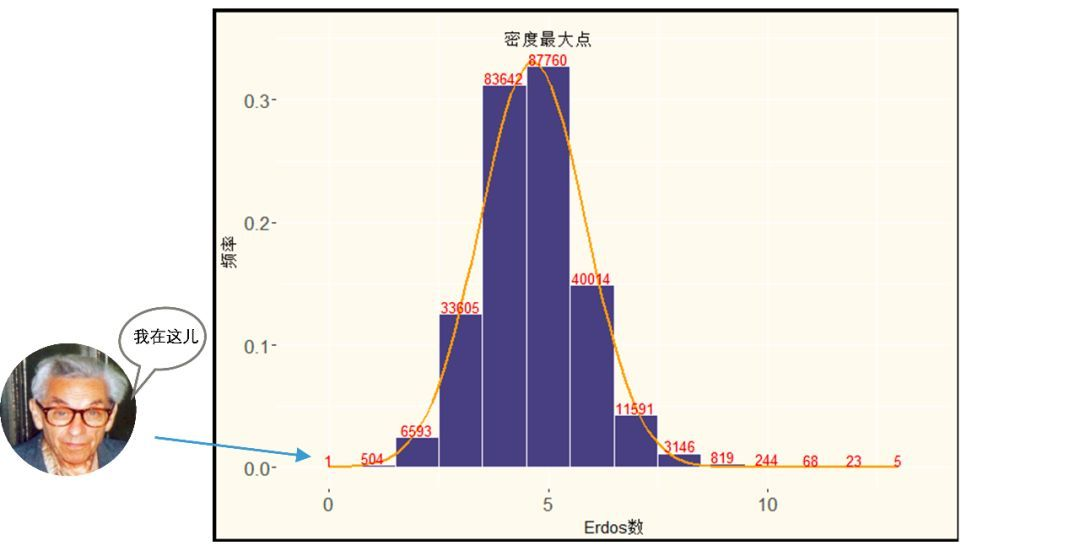
\includegraphics[width=0.8\textwidth]{figure/erdosNumber.jpeg}
        \caption{有限 Erdos 数分布}
        \label{fig:my_label}
    \end{figure}
\end{frame}

\section{写作前:构建雏形}
\begin{frame}{写作前:构建雏形}
    \flushleft{\textit{According to this technique, one does not write the paper in linear order, and one also refrains from
the temptation of writing the easiest or most straightforward portions first. \\ \ \\  根据这种技术,人们不会以线性顺序书写论文,而且还避免了先写最容易或最直接的部分的诱惑。}} \\ 
\flushright{\cndash Terence Tao\footnote{陶哲轩(1975-), 华裔数学家, 菲尔茨奖获得者, 21岁获得普林斯顿大学博士学位,  24岁起在加利福尼亚大学洛杉矶分校担任正教授}, \textit{Write a rapid prototype first.}}
\end{frame}

\begin{frame}{写作前:构建雏形}
\begin{itemize}
\item \textcolor{blue}{你有什么} \\ \ \\
\item \textcolor{blue}{你缺什么}
\end{itemize}
\end{frame}

\begin{frame}{写作前:构建雏形}
\begin{itemize}
    \item \textcolor{blue}{写出文章的“骨架”}\\ \ \\
    \item \textcolor{blue}{写下足够多的证明} \\ \ \\
    \item \textcolor{blue}{梳理命题引理之间的逻辑}\\ \ \\
    \item \textcolor{blue}{尽可能填写论文“常规”部分}
\end{itemize}
\end{frame}

\section{写作中:如何写好论文}
\subsection{关于论文}
\begin{frame}{关于论文}
\begin{alertblock}{论文整体结构}
\end{alertblock}
        \begin{itemize}
            \item 标题 (Title)
            \item 作者 (List of authors)
            \item 摘要 (Abstract)
            \item 引言 (Introduction)
            \item 主体 (Main Part)
            \item 总结* (Conclusions)
            \item 致谢* (Acknowledgements)
            \item 文献 (References)
            \item 附录* (Appendix)
        \end{itemize}
\end{frame}

\begin{frame}{关于论文}
\begin{columns}
	\column{0.63\textwidth}
\begin{alertblock}{好的论文或许没有统一的标准}
\end{alertblock}
\textit{"作为 Advances in Mathematics 杂志的编辑,我经常将提交的论文发回给作者,并建议他们加长引言部分。有一次,我以回邮方式收到了作者的来信,说那篇论文刚被 Annals of Mathematics 以引言太长为由拒绝。"}
    \\  \flushright{\cndash Gian-Carlo Rota, \textit{Ten Lessons I Wish I Had Been Taught.}}
\begin{alertblock}{我们希望声明规范的结构, 并给出表达上的小建议}
\end{alertblock}
\column{0.37\textwidth}
\begin{figure}
    \centering
    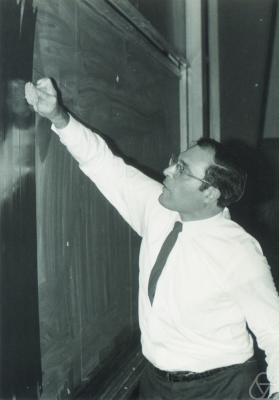
\includegraphics[width=\textwidth]{figure/rota.jpg}
    \label{fig:my_label}
\end{figure}
\end{columns}
\end{frame}

\subsection{整体建议}
\begin{frame}{整体建议: 标题 \\ Title}
\begin{alertblock}{标题应注意什么}
\begin{itemize}
    \item 应尽可能提供丰富的信息,但不要太繁琐或太长 \\
    \XSolidBrush \ \ \textit{A Decomposition of Compact Continua and Related Results on Fixed Sets under Continuous Mappings \\ \ \ \  (连续映射下固定集上紧连续性和相关结果的分解)} \\ \ \\
    \item 使用一些精炼的关键词,但不能太笼统 \\
    \XSolidBrush \ \ \textit{On a nonlinear parabolic problem from physics \\ \ \ \  (关于一个物理学的非线性抛物线问题)}\\ \ \\
    \item 避免缩写名称,避免符号 \\
    \XSolidBrush \ \ \textit{The conjecture of Budd-Smith-Watson in unframed HBK geometry  \\ \ \ \ (无框HBK几何中Budd-Smith-Watson的猜想)}
\end{itemize}
\end{alertblock}
\end{frame}

\begin{frame}{整体建议: 标题 \\ Title}
\begin{alertblock}{好标题的特征}
\begin{itemize}
    \item 生动而信息丰富: 加入动词 \\ \Checkmark \textit{Computing the eigenvalues and eigenvectors of symmetric arrowhead matrices \\ \ \ \ (对称箭型矩阵特征值和特征向量的计算)} \\ \ \\
    \item 吸引读者兴趣: 使用疑问句 \\ \Checkmark \textit{How and how not to check Gaussian quadrature formulae \\ \ \ \ (如何以及如何不检查高斯积分公式)} \\ \ \\
    \item 经典形式: 一般性说明后跟更具体的信息 \\ \Checkmark \textit{Regression Diagnostics: Identifying Influential Data and Sources of Collinearity \\  \ \ \ (回归诊断:确定有影响力的数据和共线性的来源)}
\end{itemize}
\end{alertblock}
\end{frame}

\begin{frame}{整体建议: 作者 \\ List of Authors}
\begin{alertblock}{作者署名顺序}
\textcolor{blue}{数学领域的传统是按字母顺序列出作者:} 这种传统似乎与每位作者对作品做出公平贡献的典型情况相对应,但由于这是普遍做法,因此不建议偏离此原则。
\end{alertblock}
\begin{figure}
    \centering
    
\includegraphics[width=0.7\textwidth]{figure/ratPaper.png}
    \caption{诺贝尔物理学奖得主、石墨烯发现者 A.K. Geim 的论文}
    \label{fig:my_label}
\end{figure}
\end{frame}

\begin{frame}{整体建议: 摘要 \\ Abstract}
\begin{alertblock}{摘要写作}
\begin{itemize}
    \item 摘要应尽可能提供丰富的信息,但又不要太繁琐或太长($\text{句子数}=0.3$ $\sim$ $0.5\times \text{页面数}$),保证吸引力
    \item 不用提供严格的定义和详细的结果说明
    \item 避免无用的衔接, 如 "在本文中, 除了其他事项外, 我们还证明了..."
    \item 避免使用符号和公式, 语言尽可能通俗易懂
\end{itemize}
\end{alertblock}
\end{frame}

\begin{frame}{整体建议: 摘要 \\ Abstract}
\begin{alertblock}{摘要写作}
\begin{itemize}
    \item \textcolor{blue}{文章想告诉读者什么} 
    \item \textcolor{blue}{研究这个问题的意义} 
    \item \textcolor{blue}{怎么得到结果的} 
\end{itemize}
\end{alertblock}
\begin{alertblock}{真实例子}
\textit{我们提出并分析了$\underline{\qquad}$模型中的$\underline{\qquad}$方法。$\underline{\qquad}$部分基于$\underline{\qquad}$。 对于$\underline{\qquad}$的情况,我们发现了$\underline{\qquad}$性质,并针对该情况给出了$\underline{\qquad}$。}
\end{alertblock}
\end{frame}% okk

\begin{frame}{整体建议: 摘要 \\ Abstract}
\begin{alertblock}{关键词与分类号}
\begin{itemize}
    \item \textcolor{blue}{关键词:让读者预见你文章的内容}
    \item \textcolor{blue}{分类号:反映论文的研究方向}: Mathematical Reviews 数学学科分类(2020)将数学分为64个部分,并进一步分为许多小类。例如 05A20 代表组合学中的组合不等式,65F05代表数值线性代数中求解线性系统的直接方法
\end{itemize}
\end{alertblock}
\end{frame}


\begin{frame}{整体建议: 引言 \\ Introduction}
\begin{alertblock}{引言的内容} 
\begin{enumerate}
    \item 阐述研究的问题和研究的内容
    \item 关键困难在于何处
    \item 相关工作以及最先进的结果(State of the art, SOTA) \\ \ \\
    \item 本文创新性点
    \item 主要的思路(证明过程、实现算法)\\ \ \\
    \item 最后概述文章的逻辑结构
\end{enumerate}
\end{alertblock}
\end{frame}

\begin{frame}{整体建议: 主体 \\ Main Part}
\begin{alertblock}{注意事项}
\begin{itemize}
    \item 分几部分组织论文,应包含符号定义,完整证明,数值实现等内容\\ \ \\
    \item 将冗长的证明分为几个步骤或几个引理\\ \ \\
    \item 注意编号,长篇论文建议采用双编号(如5.2)\\ \ \\
    \item 写作过程中注意逻辑流程\\ \ \\
    \item 尝试简化证明或描述方式
\end{itemize}
\end{alertblock}
\end{frame}


\begin{frame}{整体建议: 主体 \\ Main Part}
\begin{alertblock}{结构示例}
理论型或数值方法型论文结构有所不同: 
\end{alertblock}
\begin{columns}
\column{0.5\textwidth}
\begin{itemize}
    \item 引言 
    \item 符号定义 (有时将引理定理列在此后)
    \item 定理1证明 
    \item 定理2证明
    \item 定理3证明
    \item 拓展
\end{itemize}
\column{0.5\textwidth}
\begin{itemize}
    \item 引言
    \item 符号定义和算子
    \item 数值算法格式和主要结果
    \item 解的存在性
    \item 解的唯一性
    \item 算法的收敛性分析
    \item 数值实验
\end{itemize}
\end{columns}
\end{frame}

\begin{frame}{整体建议: 总结 \\ Conclusions}

\begin{itemize}
    \item 总结部分并非必要
    \item 如果有一个总结部分,则不应简单地用相同的单词重复前面已有的内容, 应该提供另一种观点,讨论工作的局限性,或者为进一步的研究提出建议
\end{itemize}
\end{frame}

\begin{frame}{整体建议: 致谢 \\ Acknowledgements}
在参考文献之前,在论文末尾加一个短的未编号部分, 可以使用较小的字体. Rota 建议“\textit{给予充分的感谢}”, 但也可以精炼一些。

\begin{figure}
    \centering
    
\includegraphics[width=\textwidth]{figure/ackPic.png}
    \caption{\textit{On non-uniqueness of percolation on nonamenable Cayley graphs}, Igor Pak et al.}
    \label{fig:my_label}
\end{figure}
\end{frame}

\begin{frame}{整体建议: 致谢 \\ Acknowledgements}
在感谢所有人的同时,仍然需要做出选择, 按重要性递增的顺序进行。
\begin{alertblock}{三种类型}
\begin{enumerate}
    \item \textcolor{blue}{感谢写作过程中讨论的人},按名称的字母顺序排列。"感谢 Albert 、Bob提出的修改建议。"
    \item \textcolor{blue}{挑出提供重要建议的人重点感谢}: “特别感谢 Adam Smith 介绍的引理, 这一结果在第 3 节的分析中起了简化作用。" 
    \item \textcolor{blue}{感谢所在的机构以及提供资助等帮助的机构}: 
\end{enumerate}
\begin{alertblock}{学位论文记得感谢家人的支持}

\end{alertblock}
\end{alertblock}
\end{frame}


\subsection{细节建议}
\begin{frame}{参考文献引用}
    \begin{alertblock}{重要性}
    \end{alertblock}
     思考:我们为什么要写论文?
\end{frame}

\begin{frame}{参考文献引用}
    \begin{alertblock}{如何引用参考文献}
    \end{alertblock}
    \begin{itemize}
          \item 在论文最后列出你所引用的全部资料
          \item 把引用的论文标题写全,期刊名可以使用缩写
          \item 引用书籍中内容时,一定要给出具体页码
    \end{itemize}
\end{frame}

\begin{frame}{参考文献引用}
    \begin{alertblock}{如何引用参考文献} 
    \end{alertblock} 
    \begin{itemize}
        \item 公理不需要你提供参考文献
        \item 避免这样的引用:A.Friend.Private communication,2014
        \item 引用没有公开发表的论文,可以提供网页链接
    \end{itemize}
\end{frame}

\begin{frame}{参考文献引用}
    \begin{alertblock}{如何引用参考文献} 
    \end{alertblock} 
    \begin{itemize}
        \item 不同的帮助程度,不同的表述方式
        \item 引用一系列文章时,根据贡献大小依次排列
        \item 引言中最好引用最相关的论文,尽量不要在论文主体部分加入大段的引用
    \end{itemize}
\end{frame}

\begin{frame}{写作细节}
\begin{alertblock}{表达清晰}
    \begin{itemize}
    \item \textcolor{blue}{不明确的指代}: “ A具有属性Y但不具有Z,此属性允许它执行某操作”
    \item \textcolor{blue}{复杂逻辑结构}:“如果X和Y或Z然后P或Q”
    \item \textcolor{blue}{数学符号和文本的混合}
    \item \textcolor{blue}{繁琐的符号}: $M_{i_{j, k_{t}}}^{O_{b}^{c}}$, 或是一个使用 $(a, b, c, d, e, f, g, h, i, j)$ 定义的系统
    \end{itemize}
\end{alertblock}
\end{frame}

\begin{frame}{写作细节}
    \begin{alertblock}{页面布局清晰明了,数学公式和文字的比例适当}
    \end{alertblock}
    \begin{itemize}
        \item 数学公式过多:读者难以理解
        \item 文字叙述过多:不简练,没有体现出数学论文的特色
    \end{itemize}
\end{frame}

\begin{frame}{写作细节}
\textbf{公式和方程式必须包含在带有适当标点符号的完整句子中}\par
面包店总收入$R$的计算公式为:
$$R=pq,$$
这里$p$是面包的价格,$q$是卖出面包的数量,根据历史经验当每个面包定价15元时,可以卖出2000个面包。同时,面包价格每增加1元,将会少卖出150个面包。因此如果面包价格上升$x$元,则收入为:
\begin{align*}
    R&=(15+x)(2000-150x)\\
   &=-150x^{2}-250x+30000.
\end{align*}
\end{frame}

\begin{frame}{写作细节}
\textbf{重要的或较长的公式应该单独成行,比较以下两种写法:}\par
\begin{enumerate}
    \item 令$d$为Bob距离地面的距离,$t$为Bob落地的时间,$d$与$t$满足关系式$d = 100 − 16t^{2}$。我们求解方程$100 − 16t^{2} = 0$,解得$t =2.5$,因而Bob将在2.5秒后落地。\par
    \item 令$d$为Bob距离地面的距离,$t$为Bob落地的时间,$d$与$t$满足关系式:
         $$d = 100 − 16t^{2},$$
         我们求解以下方程:
         $$100 − 16t^{2} =0,$$
         解得$t =2.5$,因而Bob将在2.5秒后落地。
\end{enumerate}
\end{frame}
\begin{frame}{写作细节}
    \begin{alertblock}{不要钻牛角尖}
    \end{alertblock}
    当涉及到标准或简单的概念时,多余的解释会分散读者注意力,并使论文不太清楚,例如当你用一些图形覆盖一个区域时,没有必要很详细地叙述你是如何不重叠完全覆盖这个区域的,可以用一幅图来代替。
\end{frame}

\begin{frame}{写作细节}
    \begin{alertblock}{关于插图}
    \end{alertblock}
    可以适当多一些图片,但是需要控制图片的大小,如果图片过大,包含的细节太多,会破坏阅读论文的流畅性,如果很有必要使用这种类型的图片,可以把它们放到附录里。
\end{frame}
    
\begin{frame}{写作细节}
    \begin{alertblock}{句子长短}
    \end{alertblock}
    尽量避免使用很长的句子,有些句子从语法的角度看是不需要用逗号隔开的,但是你仍然可以用逗号隔开,这样做一定程度上让读者更容易理解句子的意思,同时不要过多使用逗号,否则会影响文章的流畅性。
\end{frame}

\begin{frame}{写作细节}
\begin{alertblock}{数学符号}
\end{alertblock}
    \begin{itemize}
        \item 相同的符号不能用来表示不同的东西
        \item 所有的变量第一次出现的时候都要进行解释说明
        \item 使用标准的,公认的符号
        \item 某一符号隔了好几页再次出现,记得再次进行解释
    \end{itemize}
\end{frame}

\begin{frame}{写作细节}
    \begin{itemize}
        \item 不要随意更改专业术语,特别是进行英文写作
        \item 不要避讳使用第一人称
        \item 不要用符号或者公式作为一个句子的开头\par
        \kaishu{$x^{n}-a$有$n$个不同的零点。}\par
        \kaishu{多项式方程$x^{n}-a$有$n$个不同的零点。}
    \end{itemize}
\end{frame}

\begin{frame}{写作细节}
\begin{itemize}
    \item 在文字论述时,不要使用数学符号代替汉字,比如用$\because$代替因为,用$\therefore$代替所以
    \item 把论文分成几个部分,读者可以更容易地找到方程和定理\par
    \kaishu{根据定理31,我们可以证明......}\par
    \kaishu{根据定理4.3,我们可以证明......}
\end{itemize}
\end{frame}

\section{写作后:自我检查}
\begin{frame}{Checklist}
    \begin{figure}
        \centering
        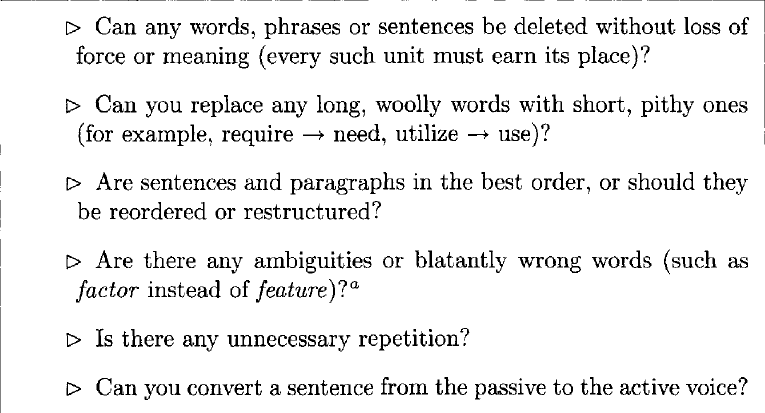
\includegraphics[width=0.9\textwidth]{figure/Figure 7_1_1.png}
        \label{fig:my_label}
    \end{figure}
\end{frame}

\begin{frame}{Checklist}
    \begin{figure}
        \centering
        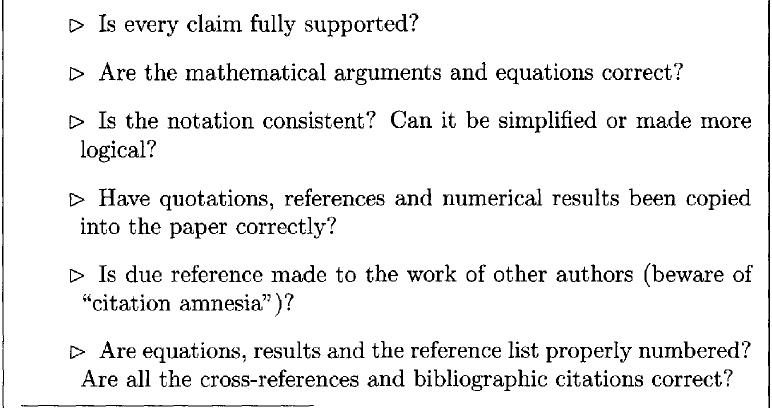
\includegraphics[width=0.9\textwidth]{figure/Figure 7_1_2.png}
        \label{fig:my_label}
    \end{figure}
\end{frame}

\begin{frame}{Checklist}
    \begin{figure}
        \centering
        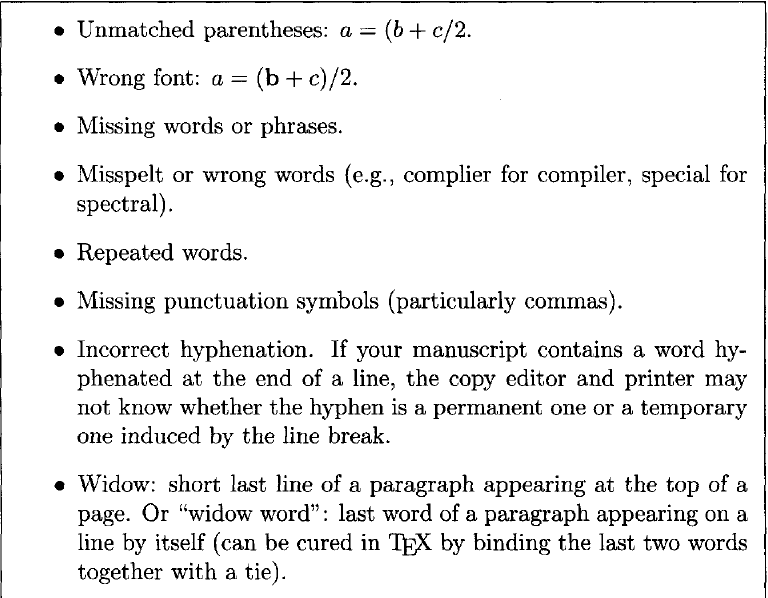
\includegraphics[width=0.9\textwidth]{figure/Figure 8.2.1.png}
        \label{fig:my_label}
    \end{figure}
\end{frame}

\begin{frame}{Checklist}
    \begin{figure}
        \centering
        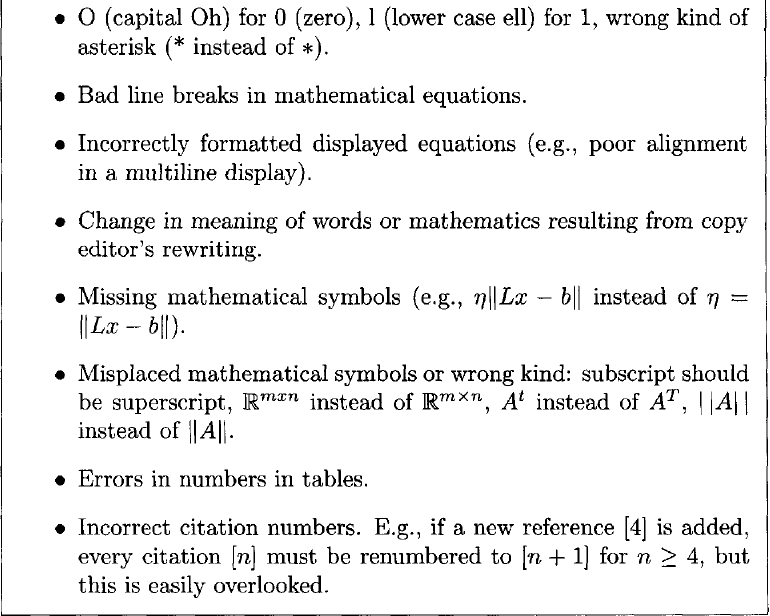
\includegraphics[width=0.9\textwidth]{figure/Figure 8.2.2.png}
        \label{fig:my_label}
    \end{figure}
\end{frame}


\section{论文部分总结}
\begin{frame}
    \begin{itemize}
        \item 千里马常有,而伯乐不常有
        \item 学会在学术研究中形成自己的想法并与他人分享
        \item 论文的发表、讨论往往会带来新的见解和新的合作
        \item 预祝大家取得成功
    \end{itemize}
\end{frame}

\section{辅助工具}
\begin{frame}{查资料: 如何快速了解一个主题?}
\begin{alertblock}{大家如何查找资料?}
    \begin{itemize}
        \item 给了一篇论文?
        \item 给了一个主题?
    \end{itemize}
\end{alertblock}
\end{frame}

\begin{frame}{查资料: 如何快速了解一个主题?}
\begin{alertblock}{需要突破口}
    \begin{itemize}
        \item 给了一篇论文 $\xrightarrow{}$ 已有突破口\\ \ \\
        \item 给了一个主题 $\xrightarrow{}$ 寻找突破口
        \begin{itemize}
            \item Bing 搜索 "关键词 + filetype: pdf"
            \item 没有合适的关键词? 问老师, 问同学
            \item 技巧: 找 .edu 域名, 教师主页下的文章
        \end{itemize}
    \end{itemize}
\end{alertblock}
\begin{alertblock}{从突破口往下寻找引用的文献}
\end{alertblock}
\end{frame}


\begin{frame}{查资料: 如何快速了解一个主题?}
\begin{alertblock}{已有突破口: 从参考文献寻找全文}
常用全文数据库:
    \begin{itemize}
        \item 中文: \textbf{知网}(全面) > 维普 > 万方 (也有外文文献) 
        \item 英文: 
        \begin{itemize}
            \item 已发表: ScienceDirect (Springer), EBSCO (综合), PQDT (ProQuest 的学位论文库) 
            \item 预印(Preprint): \textbf{arXiv} (计算机, 数学, 物理; Cornell), medRxiv (医学; Yale) 
        \end{itemize}
    \end{itemize}
\end{alertblock}
\begin{alertblock}{但英文论文有更简便好用的方式}
\end{alertblock}
\end{frame}

\begin{frame}{查资料: 如何快速了解一个主题?}
\begin{alertblock}{从参考文献寻找全文}
引文索引平台(导航):
    \begin{itemize}
        \item 综合类: Web of Science, Scopus 
        \item 分学科: \textbf{MathScient (数学)}, DBLP (计算机)
        \item 搜索引擎: 
        \begin{itemize}
            \item 中文: 百度学术? Bing学术?
            \item 英文: Google Scholar, \textbf{Semantic Scholar(推荐)}
        \end{itemize}
    \end{itemize}
\end{alertblock}
\begin{alertblock}{主要感受: 需要校园网\&有的校园网内也访问慢}
\end{alertblock}
\end{frame}

\begin{frame}{查资料: 如何快速了解一个主题?}
\begin{alertblock}{Semantic Scholar\footnote{www.semanticscholar.org} 分析文献}
优势: 免费(无需校园网)且速度稳定
    \begin{itemize}
        \item 搜索标题或作者 (可以看到文章影响力趋势, "热点问题")
        \item 找该论文之前(引用), 之后的研究(被引)
        \item 若想要进一步了解主题:
        \begin{itemize}
            \item 相关类似作者, 推荐的相似论文
            \item 作者受谁影响大? 受谁的什么文章影响最大?
            % \item 作者对谁影响大? 哪篇文章对别人影响最大?
        \end{itemize}
    \end{itemize}
\end{alertblock}
\end{frame}

\begin{frame}{查资料: 如何快速了解一个主题?}
\begin{alertblock}{Semantic Scholar 获取全文}
    \begin{itemize}
        \item 导航平台直接导向pdf文件 (arXiv等)
        \item 导向出版商/数据库官方: 学校已购买大部分
        \item 特殊情况(学校未购买): SciHub\footnote{https://scihubtw.tw/(可能经常变)}
    \end{itemize}
\end{alertblock}
另外, 电子书可以去 Library Genesis\footnote{https://libgen.is/}
\end{frame}

\begin{frame}{资料整理: 如何管理文献?}
当已经下载了很多文献后, 需要良好的管理
\begin{alertblock}{Zotero\footnote{www.zotero.org}}
免费开源软件, 常用功能:
    \begin{itemize}
        \item 管理文献, 支持多种类型 
        \item 扫描已有 pdf 
        \item 从不同来源直接添加 (知网, Semantic Scholar, 博客网页)
        \item 阅读笔记 Markdown
        \item 加标签, 按标签分类
        \item 方便导出 .bib 文件或其他引用方式
        \item 多设备同步, 方便 Pad 做笔记
        \item 支持共享文献
    \end{itemize}
\end{alertblock}
\end{frame}

\begin{frame}{开始写作: 如何高效合作?}
本人尝试过的: Overleaf, Git, 网盘共享文件夹, 最想推荐:
\begin{alertblock}{Overleaf\footnote{www.overleaf.com}}
一个使用LaTeX进行在线、合作编辑的平台
    \begin{itemize}
        \item 不用配置环境了, 在线编译
        \item 可以邀请多位合作者同时编辑
        \item Review 批注功能
        \item 可以留 Comments 与合作者沟通
        \item History 版本对比
        \item 只带 Pad 也可以合作
    \end{itemize}
\end{alertblock}
\end{frame}

% \begin{frame}{\textbf{查资料}}

% \begin{figure}
%     \centering
%     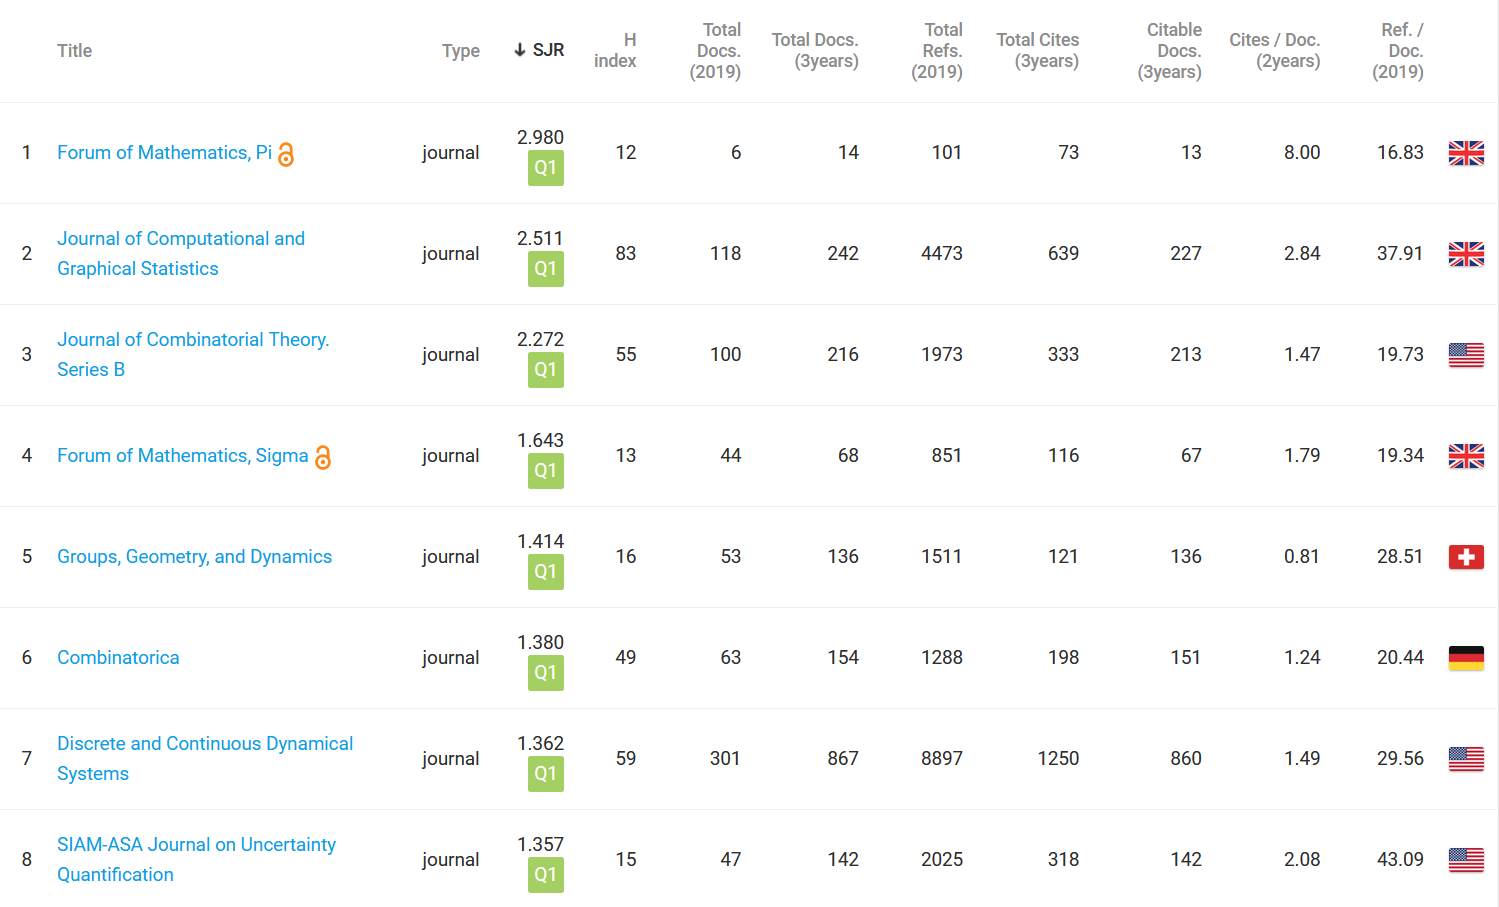
\includegraphics[width=0.95\textwidth]{figure/combRank.png}
%     \caption{组合数学期刊排行榜\footnote{www.scimagojr.com}}
%     \label{fig:my_label}
% \end{figure}
% \end{frame}


% \begin{frame}{\textbf{查资料}}

%     \begin{figure}
%     \centering
%     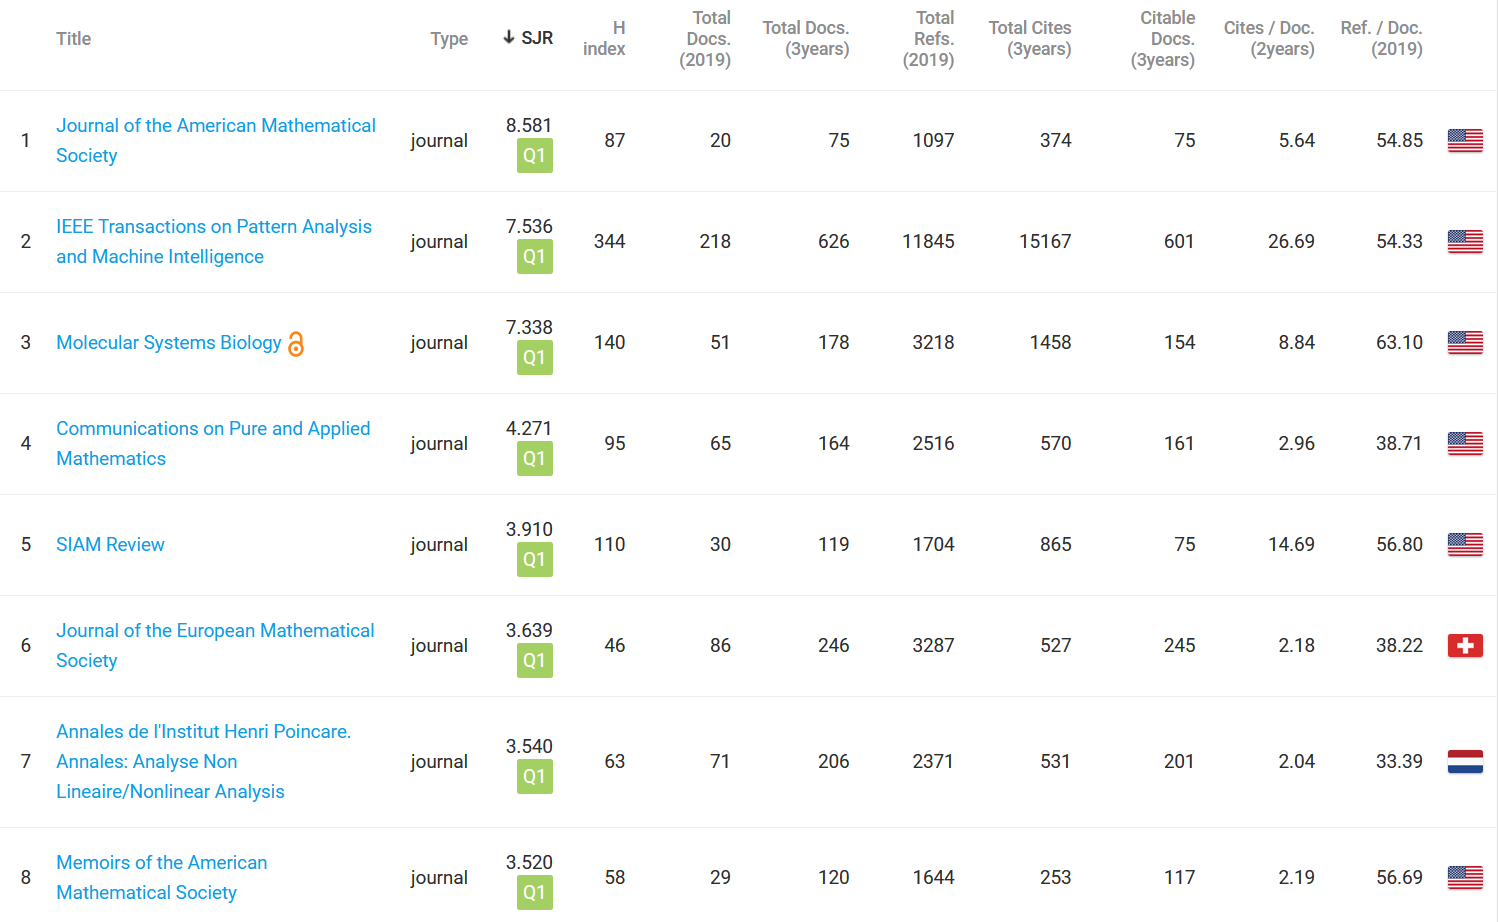
\includegraphics[width=0.95\textwidth]{figure/applRank.png}
%     \caption{应用数学期刊排行榜\footnote{www.scimagojr.com}}
%     \label{fig:my_label}
%     \end{figure}
% \end{frame}

\section{辅助工具总结}
\begin{frame}{\textbf{总结}}
    \begin{itemize}
        \item 主要是展示功能, 具体使用大家可以动手尝试
        \item 欢迎大家分享更多 "生产力工具", 辅助课程论文和毕业论文的顺利完成
    \end{itemize}
\end{frame}

\begin{frame}
    \begin{center}
        {\Huge\calligra Thank you for your attention!}
    \end{center}
\end{frame}


\end{document}


